\chapter{Introduction: Bitcoin Mining and Energy}

Bitcoin mining turns electricity into security: every block on the Bitcoin ledger carries proof that real energy was spent to make it. That proof comes at a hefty price. As of August 2026, this book estimates that the machines of the global Bitcoin mining network draw between about 147 and 212 terawatt-hours (TWh) of electricity a year, roughly 0.46 to 0.66~percent of the world's 2025 electricity generation. At the sites' meters, overhead included, the draw is 161 to 233~TWh. The range is wide because it rests on the one number in the calculation that nobody measures, the average efficiency of the machines doing the mining (Section~\ref{sec:bitcoin_consumption_own_computation}). % src: analysis/checks/ch1_network_energy.R console at 930 EH/s, "The same at the grid meter" (PUE 1.10, CBECI2026 Assumption 8): 18 J/TH = 18.41 GW = 161.3 TWh/yr = 0.50% of 32,202 TWh (EIStatReview2026); 26 J/TH = 26.60 GW = 233.0 TWh/yr = 0.72%; at the machines (the network power table): 18 J/TH = 16.74 GW = 146.6 TWh/yr; 26 J/TH = 24.18 GW = 211.8 TWh/yr; the headline is at the machines, the basis of the J/TH range, with the meter figure second (author decision 2026-09-27; the DATA-017 review round had put the meter first, because world generation is a grid-side quantity; the meter share, 0.50 to 0.72%, is printed with the comparison below); the 18 to 26 J/TH range is the author's judgment, set out in the section cited (DATA-017, 2026-09-26); until then this sentence printed 212 TWh at an assumed 26 J/TH and ranked it 25th among countries on Ember's yearly data, a neighbour pair that held only near the old single figure; across 147 to 212 TWh the rank moves by several places, so the ranking was dropped rather than printed as a range
This massive energy consumption is essential for securing the network, but it also makes mining success depend directly on access to large amounts of electrical power. In simple terms, miners are converting electricity into bitcoins, using computational work to earn digital currency rewards. In that sense, bitcoin behaves like electrified gold: a scarce commodity whose marginal production cost is dominated by energy. This book explores how energy-intensive Bitcoin mining can help power systems by providing demand flexibility, absorbing excess generation, and participating in grid stability programs.

If you already run miners, skip ahead to the efficiency of a single machine, on page~\pageref{par:ch1-efficiency}, and then go on to Chapter~2, which explains the grid.

\section{How Bitcoin Mining Works}

Bitcoin is a decentralized digital currency, and mining is the mechanism that secures its ledger. Mining achieves consensus through a protocol called \glossaryterm{proof-of-work}{Proof-of-Work (PoW)}, which Satoshi Nakamoto's Bitcoin whitepaper built on Adam Back's earlier Hashcash scheme \autocite{Nakamoto2008}. % src: Nakamoto2008 sec. 4, Proof-of-Work: "we will need to use a proof-of-work system similar to Adam Back's Hashcash"; until 2026-10-10 this line said PoW was "originally outlined by Satoshi Nakamoto" (review comment: PoW predates Bitcoin)

In PoW mining, specialized computers (``miners'') compete to solve a cryptographic puzzle by repeatedly hashing data for a \glossaryterm{bitcoin-block}{block}, a batch of transactions proposed for addition to the blockchain. Hashing means running data through a one-way function that turns any input into a fixed-length number: the same input always gives the same number, a slightly different input gives an unrecognizably different one, and nobody can work backward from the number to the input. In practice, miners try to guess a number (called a \textit{nonce}) such that the resulting hash value falls below a defined target threshold. Solving this puzzle requires energy: miners must perform trillions of hash computations per second. The first miner to find a valid solution broadcasts it to the entire network. The solution itself proves the miner did the work. Miners check the transactions they put into a block, because a block containing an invalid one would be rejected and its reward lost, but the final say belongs to the independent nodes that check every block against the rules \autocite{Nakamoto2008}. % src: Nakamoto2008 sec. 5, Network, step 5: "Nodes accept the block only if all transactions in it are valid and not already spent" (review comment 2026-10-12: miners propose blocks and supply the proof of work; nodes enforce the rules)
In return, the successful miner receives a \glossaryterm{block-reward}{block reward} consisting of newly minted bitcoins and any transaction fees from the processed block. This reward keeps miners investing in powerful hardware and electricity, and that investment secures the Bitcoin network.

As bitcoin's popularity and market value have risen, mining has become increasingly competitive and resource-intensive. The network automatically adjusts mining difficulty approximately every two weeks (specifically every 2,016 blocks), targeting an average block time of roughly 10 minutes. If miners add more computational power (known as hashrate) and discover blocks too quickly, the protocol raises the difficulty level. Conversely, if hashrate falls and blocks are found more slowly, difficulty is reduced.

This self-balancing mechanism has triggered a technological arms race in mining hardware. While early miners could participate using standard desktop computers, today's mining relies on specialized machines known as \glossaryterm{asic}{ASICs} (Application-Specific Integrated Circuits). These ASICs are designed to maximize mining efficiency. They perform vast numbers of hashes per second and consume substantial amounts of electricity. The more hashing power miners collectively dedicate, and so the more hardware and electricity an attacker would have to match, the more secure, and the more expensive to attack, the Bitcoin network becomes.

\begin{figure}[h]
  \centering
  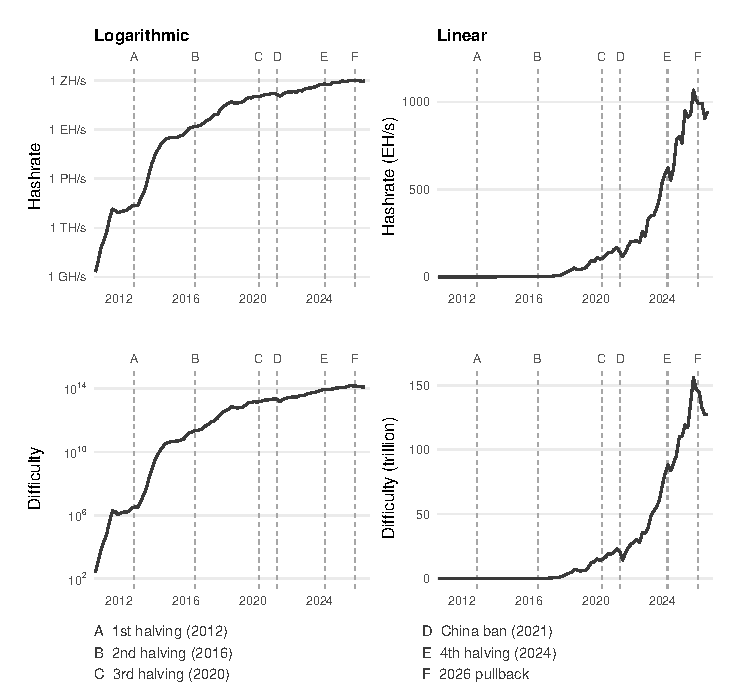
\includegraphics[width=\textwidth]{images/network_hr_diff_v2}
  \caption{
    Bitcoin network hashrate and difficulty on logarithmic scales (left) and linear scales (right). The logarithmic view spans gigahashes to zettahashes per second; the linear view shows the absolute size of rises and falls. Dashed lines mark the four halvings, the China ban and the 2026 pullback, identified by the shared key. Lines join sampled observations, which can miss short-lived peaks and troughs. Data: Braiins Insights API \autocite{BraiinsInsights}. % fig-src: analysis/figures/fig_ch1_network_hr_diff.R
  }
  \label{fig:network-hashrate-difficulty}
\end{figure}

Hashrate and mining difficulty exhibit a near-perfect correlation over Bitcoin's history because increased hashrate directly triggers increased difficulty. Technological advancements, competitive economic incentives, and growing participation have driven a long-term rise in both hashrate and difficulty. The trend is not monotonic, though: as the figure shows, hashrate retreated in 2026 from a peak of roughly 1{,}100~exahashes per second (EH/s) reached in late 2025. % src: analysis/checks/ch1_hashrate_peak.R on analysis/data/network_hashrate_daily.csv in 7-day means, the estimator of the 930 EH/s below: peak 1,132.7 EH/s in the week to 2025-10-20 (daily max 1,151.5 on 2025-10-18), 2026 high 1,070.1 in the week to 2026-03-02; the figure plots braiins_hashrate_difficulty_all.json, one point about every 62 days, whose top point is 1,067.6 EH/s on 2025-11-08, inside late 2025; CoinSharesMiningQ12026 (read 2026-09-26): peak approximately 1,160 EH/s in early October 2025; the 1,086 EH/s Feb 2026 high this note cited until 2026-09-26 came from a live fetch no committed file reproduces

Several major events are annotated in the graph:

\begin{itemize}
  \item \textbf{Halvings (2012, 2016, 2020, 2024)}: These occur approximately every four years and reduce the block subsidy, the newly minted part of the block reward, by half, decreasing the issuance rate of new bitcoins.

  \item \textbf{China Mining Ban (June 2021)}: The Chinese government banned Bitcoin mining operations, prompting a large-scale migration of hashrate out of the country. This resulted in a sharp drop in both hashrate and difficulty, followed by a gradual recovery as miners relocated to new jurisdictions such as North America.

  \item \textbf{2026 Pullback}: The decline visible at the right edge of the graph. A weakening bitcoin price squeezed mining margins, and several of the largest mining operators began redirecting sites and grid capacity from Bitcoin mining toward AI and high-performance-computing workloads \autocite{CoinSharesMiningQ12026,CoreScientificQ22026,TeraWulfQ22026}. % src: CoinShares Q1 2026 (hashprice ~$63 to ~$28-30/PH/day Jul 2025-Mar 2026; >$70bn announced AI/HPC contracts across listed miners); Core Scientific Q2 2026 (colocation $136.7M vs self-mining $21.5M); TeraWulf Q2 2026 (HPC lease = 71% of revenue)
\end{itemize}

Other milestones, not directly labeled in the graph, include:

\begin{itemize}
  \item \textbf{ASIC Adoption (2013--2016)}: ASIC miners were first introduced in early 2013 (the first was the Avalon ASIC Batch 1), outperforming previous GPU and FPGA mining solutions. By 2015, ASIC dominance was complete. Mining shifted toward industrial-scale operations, and network hashrate, and thus mining difficulty, skyrocketed.

  \item \textbf{Global Expansion (2017--2020)}: Driven by rising concerns over regulatory risks and centralization in China, miners increasingly expanded to regions with favorable electricity costs and regulations. This led to substantial investment in mining infrastructure in the United States and Russia, decentralizing Bitcoin mining geographically.

  \item \textbf{Post-2021 Era}: China's ban redistributed mining capacity globally \autocite{Reuters2021,CCAF2021}, and public scrutiny of mining's environmental impact intensified, pushing operators toward renewable energy. At the same time, miners deployed far more efficient hardware (Bitmain's Antminer S19 and later S21 series), which kept hashrate growing even as margins tightened.
\end{itemize}

\section{Electricity as the Primary Mining Expense}

Electricity is mining's biggest ongoing cost. Running hundreds or thousands of mining machines 24/7 consumes enormous amounts of power, and cooling those machines to prevent overheating adds even more to the bill.

Because of this, miners are obsessed with energy prices. Profitability boils down to a simple equation: the value of the bitcoin you earn versus the cost of the electricity you use to earn it. If your electricity costs are too high, you could end up spending more on power than you make in bitcoin. Successful miners chase an all-in (delivered) rate of five cents per kilowatt-hour (kWh) or less, \$50 per megawatt-hour (MWh) in this book's units, by setting up shop in regions with cheap power or striking deals for industrial rates \autocite{CBECI2026,riot2026q1prod}. In 2025 a large West Texas mine buying at the real-time price would have paid about \$51 a megawatt-hour before its retail adder: \$42 of energy and \$9 of transmission, losses, reserves and fees (Chapter~6). Some miners even pause their machines during price spikes, and some are paid by the grid to curtail, through programs called demand response. % src: CBECI2026 methodology page, Assumption 1 (read 2026-09-27): "The average electricity price for bitcoin mining globally is constant over time and is 0.05 USD/kWh", the five cents of sec:bitcoin_consumption_own_computation; riot2026q1prod (read 2026-09-27): "All-in Power Cost - Total" 3.0c/kWh for Q1 2026 (3.8 in Q1 2025), its note 7: estimated, "Inclusive of all transmission and distribution charges, fees, adders, and taxes", and net of total power credits; 5 cents/kWh = $50/MWh; analysis/checks/ch6_btm_ledger.R console (re-run 2026-09-27), the chapter 6 table tab:btm-ledger: 100 MW at transmission voltage in Oncor's territory, 2025, 95% capacity factor; energy 42.18 = LZ_WEST 2025 mean real-time settlement point price (ERCOT MIS 13061, analysis/data/ercot_rtm15_spp_loadzones_2021on.csv.gz, the book's anchor); non-energy stack 8.83 = losses 0.91 + ancillary 0.39 + uplift including ERCOT's fee 1.38 + Rider TCRF 5.65 + distribution 0.50; delivered 51.01 with no 4CP avoidance, 45.35 with all four peaks avoided, both rows of the table; a modelled site, not an observed bill, and the retail supplier margin is excluded (private), so the $51 is printed as before the retailer's adder, unlike Riot's all-in figure, which includes adders; until 2026-09-27 this line printed "as low as $0.05 per kilowatt-hour", unsourced, and "far below what most households pay", dropped because nothing sourced it (EXEC-040)

Over time, mining settles into a balance where only those with the cheapest power and best hardware stay in the game. This drives miners to places with abundant energy, like hydroelectric dams in Canada or geothermal plants in Iceland, or even to use \glossaryterm{stranded-energy}{stranded energy} that would otherwise go unused: power generated where no transmission line or nearby customer can take it, such as the gas that oil fields would otherwise burn off in flares. Texas, whose grid this book examines in depth, has become one of the biggest of these destinations.

\subsection*{A Closer Look: Inside an Antminer S21~XP}

To understand why Bitcoin mining is so energy intensive, look inside a modern mining machine. Take the Antminer S21~XP, the air-cooled machine used throughout this book.
The device consists of:

\begin{itemize}
\item Hashboards lined with the ASIC chips that do the hashing
\item One control board
\item One power supply unit (PSU)
\item High-speed fans for cooling both the hashboards and the PSU
\end{itemize}

Bitmain rates the machine at 270 terahashes per second (TH/s). Its power rating is measured at the wall and covers the chips, the fans, the control board and the power supply's own conversion losses \autocite{bitmain2024s21xp,braiinsacademytechres}. % src: bitmain2024s21xp and braiinsacademytechres, checked 2026-09-28: air-cooled S21 XP stock hashrate 270 TH/s, power on wall 3,645 W, efficiency 13.5 J/TH; highest-rated air-cooled S21 XP variant in the supplied Braiins table, distinct from XP Hyd and XP Imm. Firmware target limits are not stock ratings.

\[
\fbox{\textbf{3{,}645~W at the wall}}
\]

For comparison:
\begin{quote}
\textit{The amount of electricity an average American household consumes over an entire day \autocite{EIAHouseholdConsumption2022}, used by a single miner in just eight hours.} % src: EIA FAQ id=97, read 2026-09-25: 10,791 kWh per residential customer in 2022 = 29.6 kWh a day; 29.6 kWh / 3.645 kW = 8.1 h. The earlier "six high-end gaming PCs" comparison had no source and was cut
\end{quote}

Industrial-scale mining farms often deploy thousands of these machines. A single site with 1{,}000 S21~XP units would require about 3.6 megawatts of power for the miners alone. % src: 1,000 x 3,645 W = 3.645 MW (bitmain2024s21xp); excludes site overhead.

\phantomsection\label{par:ch1-efficiency}Dividing power draw by hashrate gives the machine's \glossaryterm{efficiency}{efficiency}: $3{,}645~\text{W} / 270~\text{TH/s} = 13.5$ joules per terahash (J/TH), Bitmain's own rating. % src: bitmain2024s21xp (power efficiency on wall at 25 C: 13.5 J/TH)
Efficiency is the single most important specification of a mining machine, and the industry's progress is easiest to read in its steady fall: a decade ago the workhorse Antminer S9 needed roughly 100~J/TH, the S21~XP examined above needs 13.5, and the latest liquid-cooled (hydro) machines have pushed below 10 (Figure~\ref{fig:asic-efficiency}). % src: analysis/data/bitmain_flagship_efficiency.csv, one Bitmain document per row: S9 launched May 2016 (Bitmain news, July 24, 2019), 14 TH/s at 1,400 W on its spec page = 100 J/TH; S21 XP 13.5 J/TH (bitmain2024s21xp); S23 Hyd 580 TH/s at 9.5 J/TH (about 5,510 W), launched at WDMS 2025, Las Vegas, May 26-27, 2025, shipping from Q1 2026 (Bitmain on X, May 27, 2025); S23 XP Hyd 600 TH/s at 8.9 J/TH (5,340 W), launched at WDMS Global 2026, Hong Kong, August 28, 2026, shipping from November 2026 (BITMAIN Shop product page, read 2026-10-12; row in the same CSV), the lowest point of the figure
Efficiency will return throughout this book, because it sets the electricity price at which a given machine stops being profitable.

\begin{figure}[h]
  \centering
  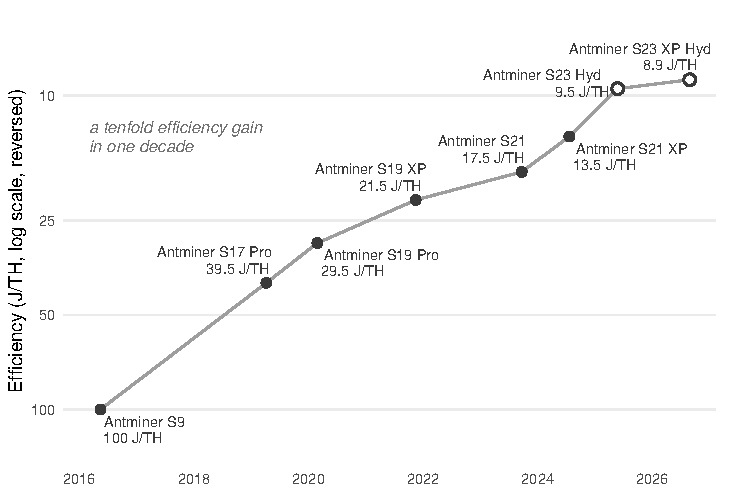
\includegraphics[width=\textwidth]{images/asic_miner_eff}
  \caption{
    ASIC miner efficiency over time: a selection of Bitmain's Antminer models at their rated efficiency at the wall on stock settings, each placed at its announcement or launch date except the air-cooled S21~XP, dated to its published specification. Lower means less energy per unit of computation; the axis is logarithmic and reversed, so the steady multiplicative gains read as a straight climb. Open points are hydro (liquid-cooled) models; filled points are air-cooled. Data: Bitmain specification pages and launch announcements, listed point by point in the companion repository. % fig-src: analysis/figures/fig_ch1_asic_efficiency.R, reading analysis/data/bitmain_flagship_efficiency.csv (one Bitmain document per point, read 2026-09-25)
  }
  \label{fig:asic-efficiency}
\end{figure}

\section[How Much Power Does Bitcoin Mining Use?]{How Much Power Does Bitcoin\\ Mining Use?}
\label{sec:bitcoin_consumption_own_computation}

To estimate the Bitcoin network's total power consumption, you need two key figures: the network's total computational throughput (hashrate) and the average energy efficiency of the mining hardware. As of August 2026, the Bitcoin network's hashrate is approximately 930~EH/s (930,000,000~TH/s) \autocite{BraiinsInsights}. % src: hashrate = 930.2 EH/s, the 7-day mean to 2026-08-21 of the committed daily cache analysis/data/network_hashrate_daily.csv (Braiins Insights global series), rounded; analysis/checks/ch1_network_energy.R reads both committed caches (analysis/data/network_hashrate_daily.csv, analysis/data/btc_price_daily.csv), 7 days to 2026-08-21. Until 2026-09-25 this cited an uncommitted live fetch of that day (927.8 EH/s)
That figure is inferred rather than counted, because nobody sees the hashes themselves: on average a block takes the difficulty times $2^{32}$ hashes to find, so dividing that by the observed time between blocks gives the network's hashrate, and a daily figure moves with the luck of how quickly that day's blocks happened to arrive \autocite{stoll2018ceepr}. % src: stoll2018ceepr p. 5 ("As each block has about 2^32 hashes, and one block is solved every 10 minutes", hashrate = difficulty x 2^32 H / 600 s); added 2026-10-12 after a review comment asking how network hashrate is estimated
The second figure is harder, because nobody measures it. Difficulty tells you how many hashes the network performs, not how many watts they cost: the protocol checks that the work was done and records nothing about the electricity it took. Every published estimate of Bitcoin's power use therefore rests on an assumption, most often an efficiency that someone modeled, and dividing such an estimate back by the hashrate returns only that assumption. % src: CCAF2025 p. 60 ("Methodologies for Estimating Electricity Consumption", four approaches, of which none measures the whole network: the top-down approach, "This widely adopted method", multiplies the implied hashrate by the assumed efficiency of a representative device; the economic approach estimates consumption "at the break-even point where mining revenue equals operational costs"; the hybrid top-down approach, CBECI's, computes the efficiency of a hypothetical device from hardware that meets a profitability threshold; extrapolation from direct measurement of "a small, representative portion of the network"; the economic approach assumes miners' operating costs, the extrapolation assumes the sample is representative; until the DATA-017 review, 2026-09-26, this sentence said every estimate multiplies the hashrate by a modelled or assumed efficiency, which the economic approach does not); CBECI2026 (FAQ, verbatim: "Bitcoin's real electricity consumption cannot be directly measured"; methodology: power = hashrate x the efficiency of a weighted basket of profitable hardware models x a PUE); protocol: the expected hashes per block are difficulty x 2^32, so difficulty fixes the hashrate and nothing on chain records power

What is published covers part of the network. Twelve fleets run by listed mining companies report their efficiency. In mid-2026 they had about 345~EH/s between them, more than a third of the network on the companies' own capacity figures, and they averaged 17~J/TH, weighted by hashrate \autocite{mara10q2026q2,bitdeer2026q2,cleanspark2026aug,riot2026q1prod}. % src: analysis/checks/ch1_fleet_efficiency.R console, section 1: 12 fleets of 11 companies, 345.1 EH/s = 37.1% of the anchor's 930.2 EH/s, 16.98 J/TH hashrate-weighted (16.65 to 17.95 across the script's variants); analysis/data/listed_miner_fleets_2026.csv, one row per fleet with its document, URL and a verbatim quote, every source re-read 2026-09-26; the four cited documents give the four largest, 235.8 EH/s: MARA 70.3 EH/s at 17.3 J/TH, Bitdeer 73.0 at 15.8, CleanSpark 50 at 16.07, Riot 42.5 at 20.2 (Riot's latest J/TH, from March)
That segment is self-reported, often from the machines' ratings rather than meters, and it leans toward efficient machines. Listed companies have the capital for the newest machines, two of them make their own, and some report the efficiency of only the machines they run, leaving out the older ones they own but have switched off. % src: analysis/data/listed_miner_fleets_2026.csv basis columns and row notes: MARA's energized hashrate assumes every operational rig is "running at 100% of manufacturers' specifications" (its 10-Q for the quarter to June 30, 2026, verbatim; row note: "Unaudited, rating-based, not metered"); Riot's fleet efficiency is "unaudited, estimated"; BitFuFu's 16.7 J/TH equals 344 MW / 20.6 EH/s, power capacity over hashrate; Bitdeer's SEALMINER and Canaan's Avalon machines; American Bitcoin's ~14.1 J/TH covers its ~58,999 operating miners of ~89,242 owned; TeraWulf's 16.4 covers its operational 5.6 EH/s of 10.6 nameplate, its whole fleet averaging 17.6

One published model of the whole fleet comes from the University of Cambridge. Nobody publishes how many of each machine were sold, so Cambridge's index takes every model still profitable at five cents a kilowatt-hour and weights it by its age; on September 25, 2026 it put the network's machines at 17.0~J/TH \autocite{CBECI2026}. % src: CBECI2026, model v1.8.0, values for 2026-09-25 read 2026-09-26: hardware efficiency 17.013 J/TH best guess (bounds 9.50 and 30.00 J/TH), power 17.12 GW with PUE 1.10 (8.78 and 32.93 GW); methodology: 0.05 USD/kWh (Assumption 1), release-date weights from 1 to 0 in steps of 0.2; FAQ: "no reliable sales or distribution figures"; quoted from CCAF material licensed CC BY-NC-SA 4.0, no CCAF data in the repository (analysis/checks/ch1_fleet_efficiency.R section 4 holds the quoted figures); until 2026-10-10 "The one published model": Coin Metrics Labs also publishes a fleet estimate (MINE-MATCH, labs.coinmetrics.io), not read or cited here
I read the model, like the listed segment, as likely to overestimate the fleet's efficiency in a lean year. Cambridge has set the model three times against miners' own reports of their fleets, and the reports have run from 3~percent more efficient than the model, in June 2022, to 11~percent less efficient, in June 2024. Cambridge expects the model to read the fleet as more efficient than it is when margins are thin \autocite{CCAF2025}, and in 2026 they were \autocite{CoinSharesMiningQ22026}. Scaled by those gaps, its 17.0 becomes 16.5 to 19.0~J/TH. % src: CCAF2025 p. 59, Figure 26(b): Bitcoin Mining Council surveys 40.6 against the model's 41.8 J/TH (June 2022) and 36.9 against 34.5 (June 2023), the CCAF survey 28.2 against 25.3 (June 2024; 45 of the survey's 49 firms, Figure 26 "Sample size: (N=45)", the survey as a whole covering nearly 48% of hashrate, pp. 9-10 and Figure 18; hashrate-weighted, which the report says leans toward the larger, more efficient firms); "CBECI estimates generally indicate slightly less efficient hardware during periods of high mining profitability and vice versa"; the direction for 2026 is the author's reading, the size is not known; CoinSharesMiningQ22026 section 1: Q2 2026 "pushed the listed mining sector below cash breakeven in aggregate", monthly average hashprice at an all-time low of $27.7/PH/s/day in June; analysis/checks/ch1_fleet_efficiency.R section 4: ratios 0.971 / 1.070 / 1.115 x 17.013 = 16.5 to 19.0 J/TH

The unknown is the rest of the network, the three-fifths that publishes no efficiency, and this book states it as a range. If the rest were nearly as efficient as the listed fleets, about 18.6~J/TH, the network would average 18; if it ran S19~Pro-class machines or worse, about 31~J/TH, it would average 26. This book takes that span, 18 to 26~J/TH at the machines, as its result. Both ends are my judgments; the listed fleets and Cambridge's model only check them. % src: analysis/checks/ch1_fleet_efficiency.R console, section 1: the rest (62.9% of 930.2 EH/s) must average 18.6 J/TH for an 18 J/TH network and 31.3 for 26 (18.4 and 29.9 if the listed share of hashes delivered is only 30%); reference machines from analysis/data/bitmain_flagship_efficiency.csv: S19 Pro 29.5, S19 XP 21.5, S21 17.5 J/TH; the range replaces the single assumed 26 J/TH of the earlier text (DATA-017, author decision 2026-09-26)

Inside that range, my own estimate is 21.5~J/TH, and it might be even lower. It is a judgment, not a measurement; it puts the rest at about 24~J/TH, and the worked example below uses it. The top of the range, 26~J/TH, would mean the fleet had made no progress since 2024: Cambridge's model already read the network's machines at 25.3~J/TH in June 2024 and at 23.7 by that December \autocite{CCAF2025}. % src: author decision 2026-09-26 (DATA-017): 21.5 J/TH is the author's current estimate, and 26 J/TH, the book's single figure until then, was set before about March 2025 (more than 1.5 years before 2026-09-26, per the author's decision of that day, which also calls it a figure for an older fleet; the prose now states that as what 26 would imply rather than as book-making history); analysis/checks/ch1_fleet_efficiency.R section 1: rest 24.2 J/TH at the listed 37.1% (23.4 at 30%); CCAF2025 pp. 59 and 63 (CBECI hardware efficiency 25.3 J/TH on 2024-06-30 and 23.7 by the end of December 2024, the book's machine basis)

Profitability puts a ceiling on the range; it cannot confirm it. At the August 2026 bitcoin price of roughly \$66{,}000 and that month's hashrate, the block subsidy pays miners about \$0.032 a day per TH/s of hashrate. % src: 450 BTC/day (144 blocks x 3.125 BTC) x $66,180 / 930.2M TH/s = $0.03202; analysis/checks/ch1_network_energy.R reads both committed caches (analysis/data/network_hashrate_daily.csv, analysis/data/btc_price_daily.csv), 7 days to 2026-08-21; transaction fees excluded (currently a low single-digit percent addition). Printed $67,000 and $0.033 until 2026-09-25, from an uncommitted fetch ($67,076, 927.8 EH/s) the repository could not reproduce
A machine paying \$50 per megawatt-hour for electricity therefore breaks even at about 27~J/TH, and one paying \$40 at about 33~J/TH; Chapter~4 derives this breakeven arithmetic in full. Machines less efficient than the breakeven for their power price mine at a loss and, sooner or later, shut down, so the operating fleet's average must sit below it. Cambridge's index draws the top of its own estimate with the same arithmetic, so the two agreeing would prove nothing. % src: analysis/checks/ch1_network_energy.R console: $0.03202/TH-day subsidy hashprice; breakeven 26.7 J/TH at $50, 33.4 at $40; 18 / 21.5 / 26 J/TH stay under the bound for a fleet paying up to $74.1 / $62.0 / $51.3 per MWh; CBECI2026 methodology: the upper bound is the least efficient model still profitable at the assumed price, times the hashrate and a PUE of 1.20; until 2026-09-26 this paragraph called the bound a sanity check that supported 26 J/TH

The site's meter lowers the ceiling further: besides the machines, it counts the site's cooling and transformer losses, a tenth more than the machines draw in Cambridge's central case \autocite{CBECI2026}. At \$42 per megawatt-hour, the 2025 average real-time price in ERCOT's West load zone (Chapter~4), a network averaging 18~J/TH would have spent about 62~percent of its August 2026 revenue on electricity, including that additional tenth. At my estimate of 21.5~J/TH, the share would have been about three-quarters; at 26~J/TH, about nine-tenths. % src: $42.18 = mean of the 35,040 15-minute real-time settlement point prices of LZ_WEST in 2025, ERCOT MIS report 13061 (analysis/data/ercot_rtm15_spp_loadzones_2021on.csv.gz; chapter-4.tex sec:sensitivity, the book's reference price, author decisions 2026-08-24 and 2026-09-04); analysis/checks/ch1_fleet_efficiency.R console, section 3 (hashprice $0.03223 per TH-day with August's 0.67% fee share; PUE 1.10, CBECI2026 methodology Assumption 8): at $42.18, 18 J/TH 62%, 21.5 J/TH 74%, 26 J/TH 90%; at PUE 1.01 the same are 57 / 68 / 82%
Six listed miners, from the efficient end of the network, spent 58~percent of their second-quarter mining revenue on electricity after curtailment credits, which would be about three-fifths at August's lower revenue per terahash \autocite{CoinSharesMiningQ22026}. Neither end is ruled out: Cambridge suggests its survey's least efficient fleets run on exceptionally cheap power \autocite{CCAF2025}, and at \$35 per megawatt-hour even 26~J/TH takes only three-quarters of revenue. % src: analysis/data/listed_miner_power_share_2026.csv (CoinShares Q2 2026 section 5.2, six fleets, 10,561 BTC: electricity net of credits 58.3% of realised revenue, BTC-weighted; Riot's and MARA's rows checked against their own documents, MARA's including hosting fees); analysis/checks/ch1_fleet_efficiency.R section 3: period-matched 61.3% on the subsidy basis (Q2 hashprice $0.03389 against the anchor's $0.03223), 59.0% on Braiins' hashprice series; 26 J/TH at $35 and PUE 1.10: 75%; CCAF2025 p. 59, on the survey's unweighted mean of 30.6 J/TH against its median of 29.5: "A plausible explanation could be the operation of older devices in regions with exceptionally low electricity costs"

\noindent Using the basic formula:
\[
\text{Power (W)} = \text{Hashrate (TH/s)} \times \text{Efficiency (J/TH)}
\]

you get, at my estimate of 21.5~J/TH and across the range:
\begin{align*}
930{,}000{,}000~\text{TH/s} \times 21.5~\text{J/TH} &= 19{,}995{,}000{,}000~\text{W} \approx 20.0~\text{GW}\\
930{,}000{,}000~\text{TH/s} \times (18\text{--}26)~\text{J/TH} &= \boxed{16.7 \text{ to } 24.2~\text{GW}}
\end{align*}

To estimate annual electricity usage:
\begin{align*}
19.995~\text{GW} \times 24 \times 365 &\approx 175~\text{TWh/year}\\
(16.74 \text{ to } 24.18)~\text{GW} \times 24 \times 365 &\approx \boxed{147 \text{ to } 212~\text{TWh/year}}
\end{align*}

These figures are the machines' own draw. At the grid meter, including the additional tenth for cooling and transformer losses in Cambridge's central case, the same range is 18.4 to 26.6~GW, or 161 to 233~TWh a year. % src: analysis/checks/ch1_network_energy.R console at 930 EH/s: 21.5 J/TH = 19,995,000,000 W = 20.0 GW x 8,760 h = 175.2 TWh/yr; 18 J/TH = 16.74 GW = 146.6 TWh/yr; 26 J/TH = 24.18 GW = 211.8 TWh/yr, boxed as 16.7 to 24.2 GW and 147 to 212 TWh (from the unrounded 16.74 GW; the rounded 16.7 x 8.76 gives 146.3); analysis/checks/ch1_fleet_efficiency.R section 2: x PUE 1.10 (CBECI2026 Assumption 8) = 18.4 to 26.6 GW, 22.0 at 21.5 J/TH; TWh at meter 161.3 / 192.7 / 233.0 at 18 / 21.5 / 26 J/TH (also analysis/checks/ch1_network_energy.R, "at the meter" line); until 2026-09-26 the chapter assumed 26 J/TH (24.2 GW, 212.0 TWh) and printed 22 to 30 J/TH as its range

\begin{figure}[h]
  \centering
  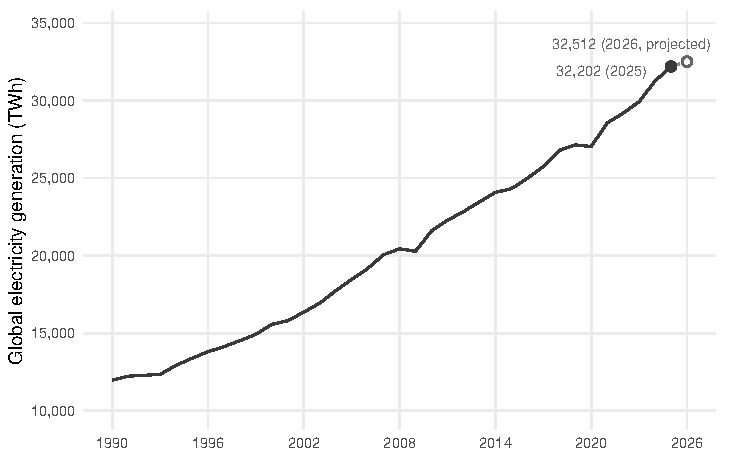
\includegraphics[width=\textwidth]{images/global_generation}
  \caption{
    Global electricity generation, 1990--2025 actuals with 2026 projected from the 2016--2025 trend. Data: Energy Institute Statistical Review of World Energy \autocite{EIStatReview2026}, 1990--2023 series as republished by Statista \autocite{StatistaGlobalGeneration2024}. % fig-src: analysis/figures/fig_ch1_global_generation.R
  }
  \label{fig:global_generation}
\end{figure}

Compare this August 2026 run-rate at the machines with global electricity generation, which reached approximately 32,202~TWh in 2025, the latest full year \autocite{EIStatReview2026}. Bitcoin mining represents:
\[
\frac{147 \text{ to } 212~\text{TWh}}{32{,}202~\text{TWh}} \times 100 \approx \boxed{0.46 \text{ to } 0.66\%~\text{of 2025 global generation}}
\]

At my 175~TWh it is 0.54~percent; at the meter, the like-for-like basis, 0.50 to 0.72~percent. % src: analysis/checks/ch1_network_energy.R console: at the machines 146.6 / 32,202 = 0.46%, 211.8 / 32,202 = 0.66%, 175.2 / 32,202 = 0.54% (the network power table); "at the meter" line (PUE 1.10): 161.3 / 32,202 = 0.50%, 233.0 / 32,202 = 0.72%, 192.7 / 32,202 = 0.60%; machines first by author decision 2026-09-27; numerator an August 2026 run-rate, denominator 2025 generation, hence the box label
By comparison, data centers used about 415~TWh in 2024, roughly 1.5~percent of global electricity consumption \autocite{IEADataCenters}. The IEA counts Bitcoin mining outside that total. % src: IEA, Energy and AI (10 April 2025), executive summary: "Data centres accounted for around 1.5% of the world's electricity consumption in 2024, or 415 terawatt-hours (TWh)". Scope: full report PDF p.71 n.2 and p.72 place cryptocurrencies (primarily Bitcoin mining, about 125 TWh in 2023, 0.5% of global electricity) outside the ICT and data centre boundary, so the 415 TWh does not double-count the 147 to 212 TWh (161 to 233 at the meter) above; the like-for-like pair is the meter figure, since both are whole-site figures (the IEA's data-centre consumption counts cooling and other infrastructure with the servers, Energy and AI p. 52: "The share of cooling systems in total data centre consumption varies from about 7% ... to over 30%", and its consumption chart splits servers, other IT, cooling and other infrastructure; the chapter's figure is at the sites' meters); the IEA's crypto figure is itself "IEA analysis based on data from ... Cambridge Centre for Alternative Finance (2025), and company reports" (Figure 2.15 sources, the CCAF entry being CBECI), so it is not a check on this chapter's range independent of CBECI2026. The earlier IEA figure of 460 TWh in 2022 (Electricity 2024) does bundle crypto and is not used here.
